\section{Introduction}
\label{sec:intro}

% ---------------- Figure 1: neuroscience analogy (safe placeholder) ----------------
% \begin{figure*}[t]
%   \centering
%   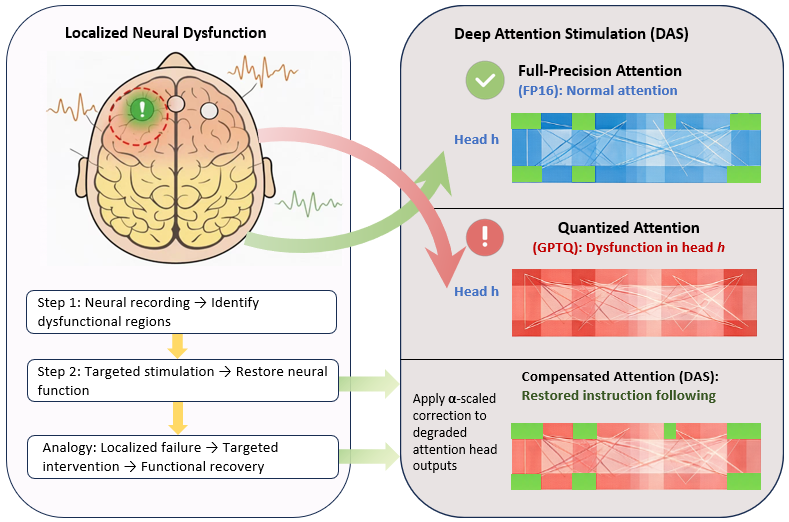
\includegraphics[width=0.8\textwidth]{figures/figure1-1.png}
%   \caption{\textbf{Neuroscience-inspired Deep Attention Stimulation.} 
%   \textbf{Left:} In cognitive neuroscience, localized neural dysfunction 
%   is diagnosed through neural recordings and remediated via targeted 
%   stimulation. 
%   \textbf{Right:} DAS applies an analogous approach to quantized LLMs. 
%   Comparing attention patterns between full-precision (FP16, top blue) 
%   and quantized models (GPTQ, middle red) identifies degraded heads 
%   (e.g., Head $h$ shows reduced attention to instruction tokens). 
%   Applying $\alpha$-scaled corrections ($\alpha \cdot \Delta\mathbf{O}$) 
%   to these heads restores attention patterns (bottom green) and recovers 
%   instruction-following capability. Heatmaps visualize attention weights 
%   where brighter regions indicate higher attention to instruction tokens.}
%   \label{fig:neuro_analogy}
% \end{figure*}
\begin{figure*}[t]
  \centering
  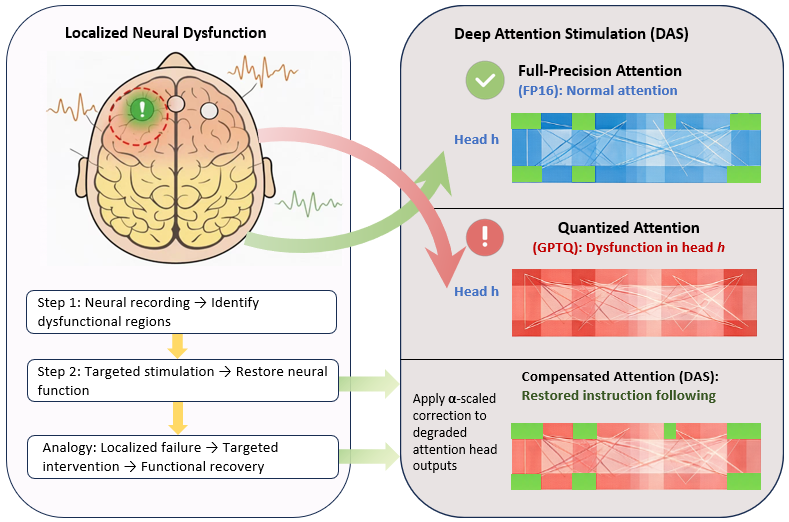
\includegraphics[width=0.8\textwidth]{figures/figure1-1.png}
  \caption{\textbf{Neuroscience-inspired Deep Attention Stimulation.} 
  Analogous to diagnosing localized neural dysfunction through recordings 
  and correcting it via targeted stimulation (left panel), DAS compares 
  attention patterns between full-precision (FP16, top blue) and quantized 
  models (GPTQ, middle red) to identify degraded heads with reduced 
  instruction token attention (right panel). Applying $\alpha \cdot \Delta\mathbf{O}$ 
  corrections to these heads restores attention patterns (bottom green) 
  and recovers instruction-following capability. Heatmaps visualize attention 
  weights where brighter regions indicate higher attention.}
  \label{fig:neuro_analogy}
\end{figure*}

Large language models (LLMs) have achieved remarkable success in instruction following, enabling users to specify complex constraints on language, format, style, and structure through natural language prompts~\citep{ouyang2022training,wei2022finetuned}. 
However, deploying such models in real-world, resource-constrained environments almost inevitably requires aggressive compression, particularly low-bit quantization~\citep{frantar2022gptq,lin2023awq}. 
While quantized LLMs can often preserve perplexity and many downstream task scores, it has been increasingly observed that instruction-following behavior degrades in subtle yet severe ways after quantization~\cite{qin2025empirical}. 
In practice, quantized models may respond in unintended languages, violate strict formatting constraints, or fall into repetitive and degenerate generations-failure modes that are poorly captured by standard evaluation metrics but critically impact usability.

Instruction following is a fragile and multifaceted capability, relying on precise coordination between semantic understanding, constraint tracking, and long-range control~\citep{zhou2023ifeval}. 
Benchmarks such as IFEval explicitly evaluate whether models adhere to lexical, structural, and stylistic constraints expressed in prompts, revealing failures that may be invisible under conventional accuracy-centric evaluations. 
Notably, quantization-induced instruction-following failures can be highly inconsistent: a quantized model may succeed on most prompts while catastrophically failing on a small subset, even when its full-precision counterpart performs correctly. 
This raises a fundamental question: \emph{are instruction-following failures under quantization the result of global degradation across the model, or do they stem from localized disruptions within specific internal components?}

Inspired by diagnostic and intervention techniques in cognitive neuroscience-particularly electroencephalography (EEG) and targeted neural stimulation-we approach this question from a mechanistic perspective~\citep{dayan2001theoretical,buzsaki2006rhythms}. 
In neuroscience, specific cognitive impairments are often traced back to dysfunction in specific brain regions rather than uniform degradation across the whole brain, enabling localized stimulation to improve or even restore functions. 
Drawing an analogy to transformer-based LLMs, we view attention heads as functional “neural clusters” whose coordinated activity underpins instruction-following behaviors. 
We hypothesize that low-bit quantization selectively disrupts a small subset of attention heads that are disproportionately responsible for maintaining instruction adherence, and that compensating these heads may recover lost functionality.

Motivated by this hypothesis, we introduce \textbf{Deep Attention Stimulation (DAS)}, 
a training-free intervention that identifies and compensates attention heads most affected by quantization.
By comparing activation patterns between full-precision and quantized models on prompts where instruction following fails, DAS isolates a small set of critical heads exhibiting the largest deviations.
During inference, we inject small corrective signals derived from these activation differences directly into the affected heads to correct the "functional loss" during quantization.
Through qualitative analysis on selected failure cases from IFEval~\citep{zhou2023ifeval}, we demonstrate that this localized intervention can recover instruction-following behavior in a 4-bit GPTQ Qwen2.5-7B-Instruct model~\citep{wang2023qwen,frantar2022gptq}, correcting erroneous language switching and mitigating degenerative repetition.
\textbf{Our current analysis on 10 samples demonstrates initial findings that instruction-following failures in quantized LLMs are not uniformly distributed but arise from localized disruptions}
(selected as representative failure cases; see Appendix~\ref{app:sample-selection}),
motivating further large-scale investigation into targeted, interpretable post-quantization repair methods.

Figure~\ref{fig:neuro_analogy} summarizes the neuroscience-inspired motivation and the two-stage diagnostic stimulation workflow of DAS.

% % ---------------- Figure 1: neuroscience analogy (safe placeholder) ----------------
% \begin{figure*}[t]
%   \centering
%   \includegraphics[width=0.8\textwidth]{figures/neuro_analogy.png}
%   \caption{\textbf{Neuroscience-inspired Deep Attention Stimulation.} 
%   \textbf{Left:} In cognitive neuroscience, localized neural dysfunction 
%   (marked with red region and !) is diagnosed via EEG recordings and 
%   corrected through targeted electrical stimulation. 
%   \textbf{Right:} DAS applies an analogous approach to quantized LLMs. 
%   Comparing full-precision (FP16) and quantized (GPTQ) attention patterns 
%   identifies degraded heads (e.g., Head $h$ shows diffused attention away 
%   from instruction tokens like ``lowercase''). These heads are compensated 
%   with $\alpha$-scaled corrective signals ($\alpha \cdot \Delta O$), 
%   restoring instruction-following capability. Both systems demonstrate 
%   how localized dysfunction can be repaired through targeted intervention 
%   rather than system-wide modification.}
%   \label{fig:neuro_analogy}
% \end{figure*}
